% ~ 6 pages
\chapter{Machine Learning}
\label{sec:ml}

Machine learning is the study of algorithms that are able to learn structure
from data (called training data) and can subsequently be used to make
predictions on unseen data. Examples for such algorithms are \emph{Boosted
  Decision Trees} (BDT) and \emph{Neural Networks} (NN) that are able to model
nonlinear problems without the need to supply an explicitly derived rule-set or
functional form. They often offer superior performance compared to linear models
or cut-based approaches at the cost of interpretability. Machine learning
techniques are commonly used for the reconstruction of hadronic tau decays in
the ATLAS experiment. Aside from tau identification they are also used for track
classification, decay mode classification and energy calibration.

The focus lies on the problem of supervised learning which is concerned with
learning models from labelled data, meaning the desired output for each example
is available during training. These problems range from regression (modelling a
dependent variable given a set of explanatory variables) to classification which
assigns a class (e.g.\ signal or background) to an observation with a set of
observed variables.

This chapter gives an overview over the techniques used in this thesis starting
with a brief description of \emph{Boosted Decision Trees} that are used in
chapter~\ref{sec:bdt} for rejection of tau candidates originating from dijet
events. A comprehensive summary on \emph{Recurrent Neural Networks} is given
that are used for tau identification in chapter~\ref{sec:rnn} and additionally
for decay mode classification in chapter~\ref{sec:decaymode}. An overview of the
software frameworks used for this thesis concludes this chapter.

\section{Boosted Decision Trees}
\label{sec:bdt}

The following section describes a classification algorithm called \emph{Boosted
  Decision Trees}. It consists of an ensemble of decision trees that is created
by a meta-algorithm called \emph{boosting}. In
section~\ref{sec:ml_decision_trees} the decision tree algorithm is presented. A
brief overview of \emph{boosting} algorithms is given in
section~\ref{sec:ml_boosting}. The description focuses on binary classification
tasks aiming to discriminate between two distinct classes (hereafter called
signal and background).

\subsection{Decision Trees}
\label{sec:ml_decision_trees}

\begin{figure}[htb]
  \centering
  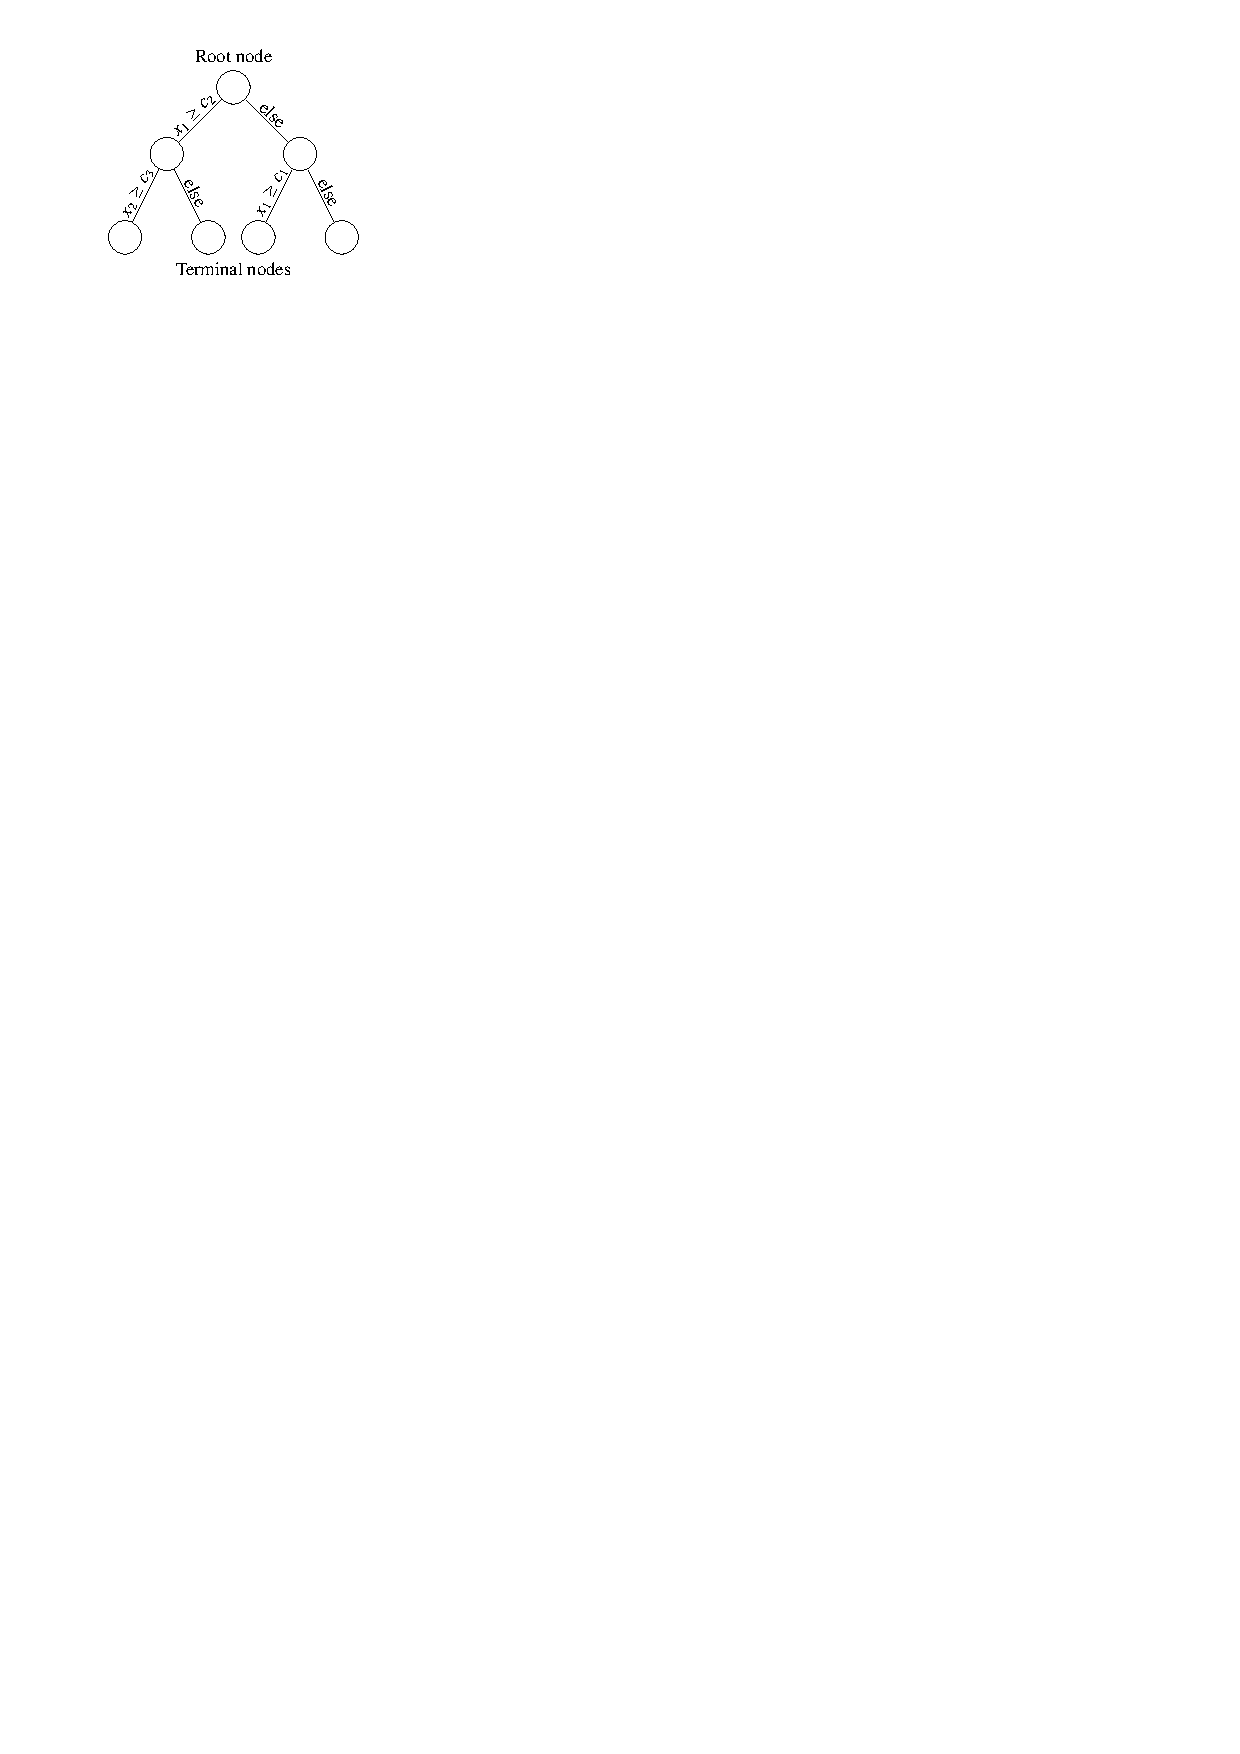
\includegraphics{./figures/theory/decision_tree.pdf}
  \caption{Binary tree structure of a decision tree. \cite{esl}}
  \label{fig:decision_tree}
\end{figure}

\todo[inline]{Dataflow not clear; Gini index: Probability to assign
  the correct label to a randomly picked observation when randomly
  assigning according to the distribution of labels in the sample
  (splits that split off pure background as well as signal are
  equivalent); Pruning?; Overfitting?}

A decision tree is a tree-based model that recursively partitions the space
spanned by the input variables into disjoint subregions by applying binary
splits on the coordinate axes until a stopping criterion is met. Frequently used
criteria include limiting the maximum depth of the tree or requiring a minimum
number of training examples in a node considered for further splitting. Figure
\ref{} illustrates the tree structure: \todo{Explain: root node - full dataset;
  node - subset; terminal node (leaf) - predicts}.

A decision tree is grown using a greedy optimisation method, where each node is
split on the variable that gives the largest improvement according to a chosen
impurity measure. Commonly used for binary classification trees is the
\emph{Gini impurity} given by
\begin{align*}
  I_\text{G}(p) = 2 p_1 p_2 = 2 p (1 - p) \qquad \text{with} \qquad p \coloneqq p_1 = 1 - p_2 \eqcomma
\end{align*}
where $p_i$ is the purity of class~$i$ \cite{esl}. The best split is
chosen such that the mean of the Gini impurities of the resulting
nodes, weighted by the sum of event weights in each node, is
minimised. Each terminal node is assigned the majority class of the
subset of training data contained within it. An alternative is to to
assign the signal purity to allow for a measure of confidence in the
decision.
% The subregions of the variable space defined by the terminal nodes Formally:
% majority class minimises classification error, signal purity minimises
% log-loss
\todo[inline]{For standalone DT -- pruning}

\subsection{Boosting}
\label{sec:ml_boosting}

Boosting describes a family of machine learning meta-algorithms that are used to
build ensembles of base classifiers which aim to improve the overall predictive
power compared to a single model. The ensembles can be viewed as an additive
expansion of the underlying functional dependence in a set of basis functions
given by the base learner \cite{esl}. Boosting is commonly used in conjunction
with Decision Trees giving rise to so called \emph{Boosted Decision Trees}.

\todo{Hyperparameter number of trees}

\emph{AdaBoost} (Adaptive Boosting) is a boosting algorithm that forms a
weighted sum of the base classifier, where each classifier is trained on data
that is reweighted such that training examples that were previously incorrectly
classified contribute with higher weight than examples that were correctly
classified. \todo{\emph{AdaBoost} $\beta$ -- learning rate -- modifies boost
  weight}

A generalisation of this method is called \emph{gradient boosting} which allows
the minimisation of an arbitrary differential loss function during boosting. A
loss function -- ya. Gradient boosting reproduces the \emph{AdaBoost} algorithm
if the exponential loss function $\exp(-f(x) y)$ is used. In general for
different loss functions no convenient methods of minimising the loss exist and
a gradient descent algorithm is used. A full mathematical description of the
algorithm is omitted for brevity and can be found in \cite{friedman_gbm, esl}.
Instead we focus on the major difference between \emph{AdaBoost} and gradient
boosting with binomial log-likelihood $\log\left( 1 + \exp(-2 f(x) y) \right)$
(TMVA) loss. Regularisation using shrinkage $\eta$.


\begin{itemize}
\item Popular algorithms: AdaBoost (TMVA: Real AdaBoost), Gradient boosting

\item AdaBoost: weighted sum of a number of weak classifiers, each classifier is
  trained on data where the weights of incorrectly classified examples are
  increased and correctly classified events are decreased

\item AdaBoost performance degrades drastically in noisy settings due to
  exponential loss function \cite{esl} binomial log-likelihood more robust
  (problems with overlapping class distributions)

\end{itemize}

\section{Neural Networks}
\label{sec:nn}

\todo{Explain notation -- bold for vectors and matrices}
\todo{Combination of different layers allow for flexible architectures}
\todo{Hidden layers -- do not interact directly with input or output but via
  intermediate nodes}

\subsection{Feedforward Neural Networks}
\label{sec:nn_feedforward}

\begin{figure}[ht]
  \begin{subfigure}[t]{0.55\textwidth}
    \centering
    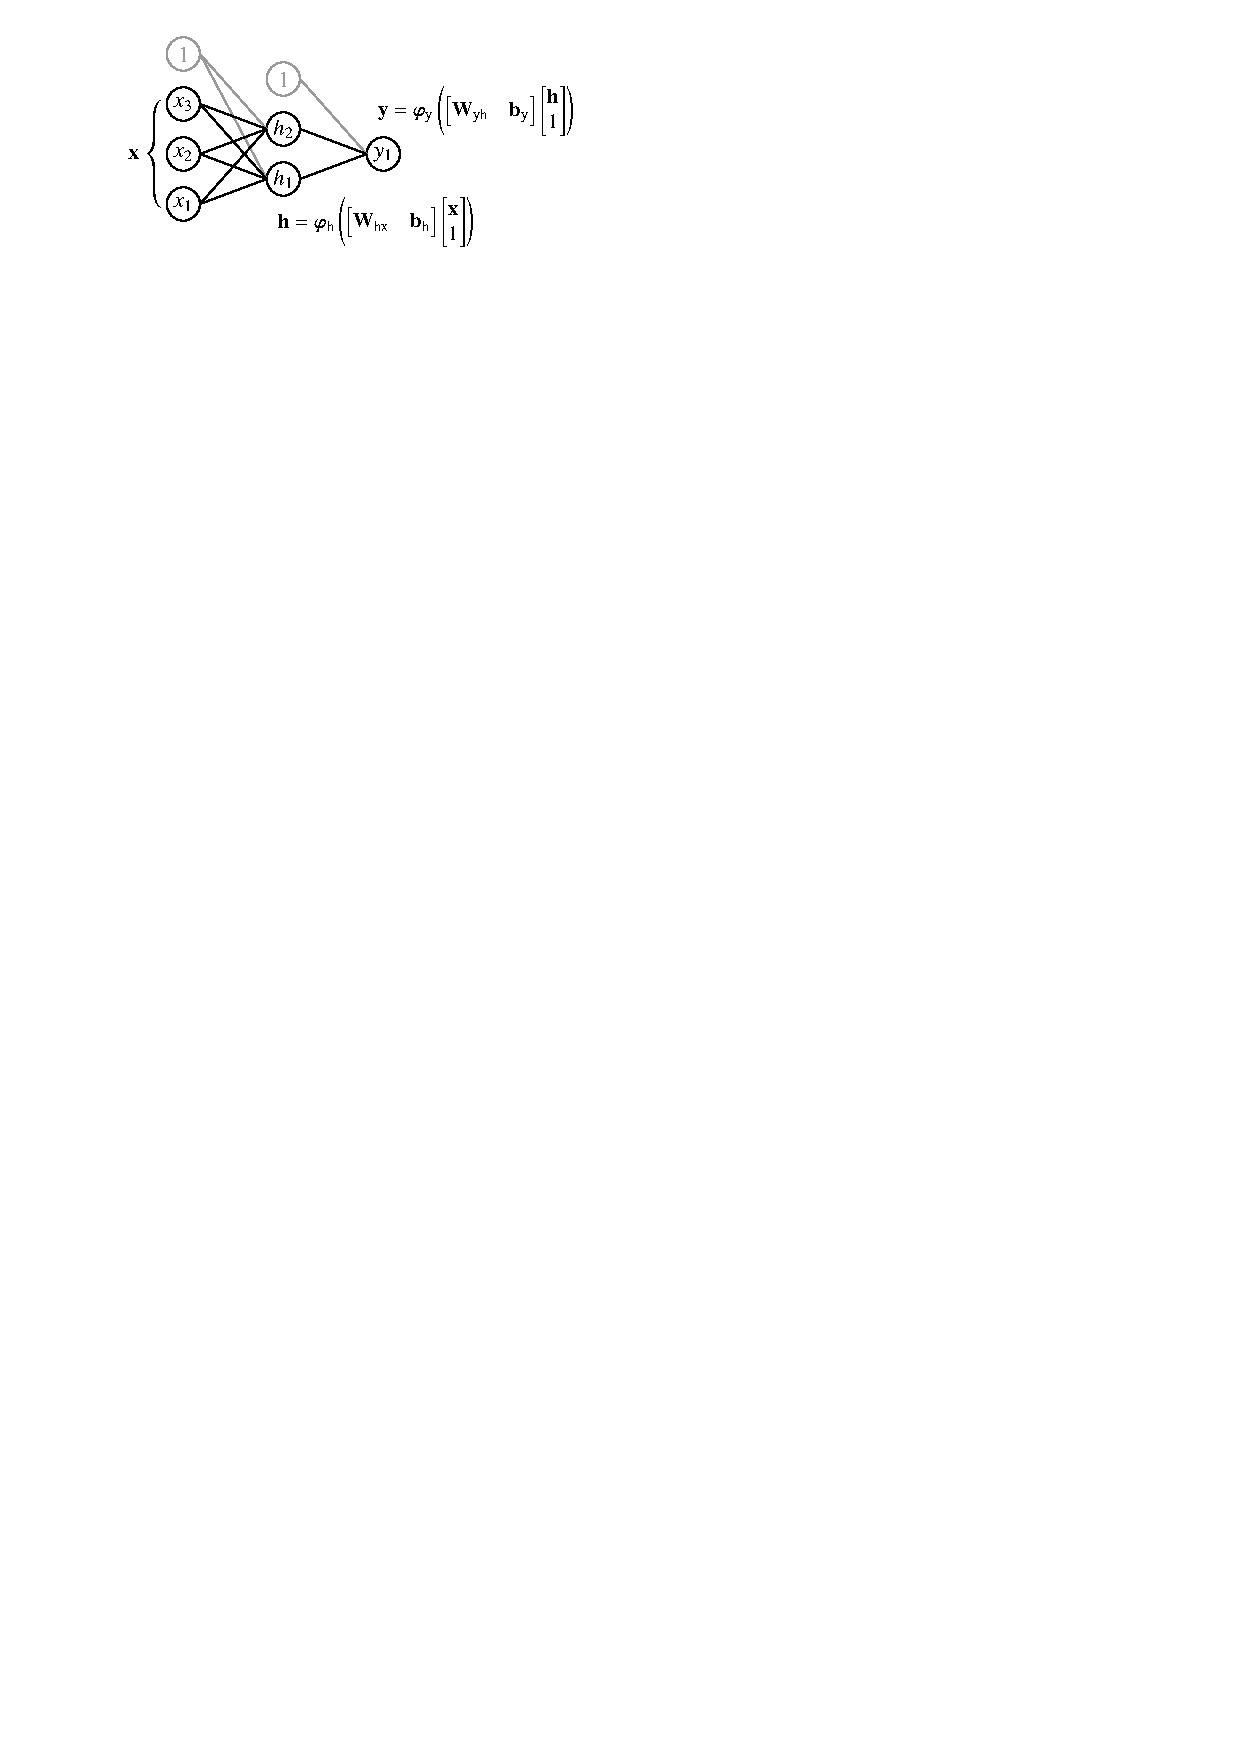
\includegraphics{./figures/theory/mlp.pdf}
    \subcaption{Schematic depiction of a multi-layer perceptron with input
      neurons $\mathbf{x}$, hidden layer activation $\mathbf{h}$ and output
      activation $\mathbf{y}$. The layers are connected via weight matrices
      $\mathbf{W}$ and optional bias vectors $\mathbf{b}$. Neuron activations
      are given after applying an element-wise activation function $\bm{\varphi}$.}
    \label{fig:multi_layer_perceptron}
  \end{subfigure}\hfill
  \begin{subfigure}[t]{0.4\textwidth}
    \centering
    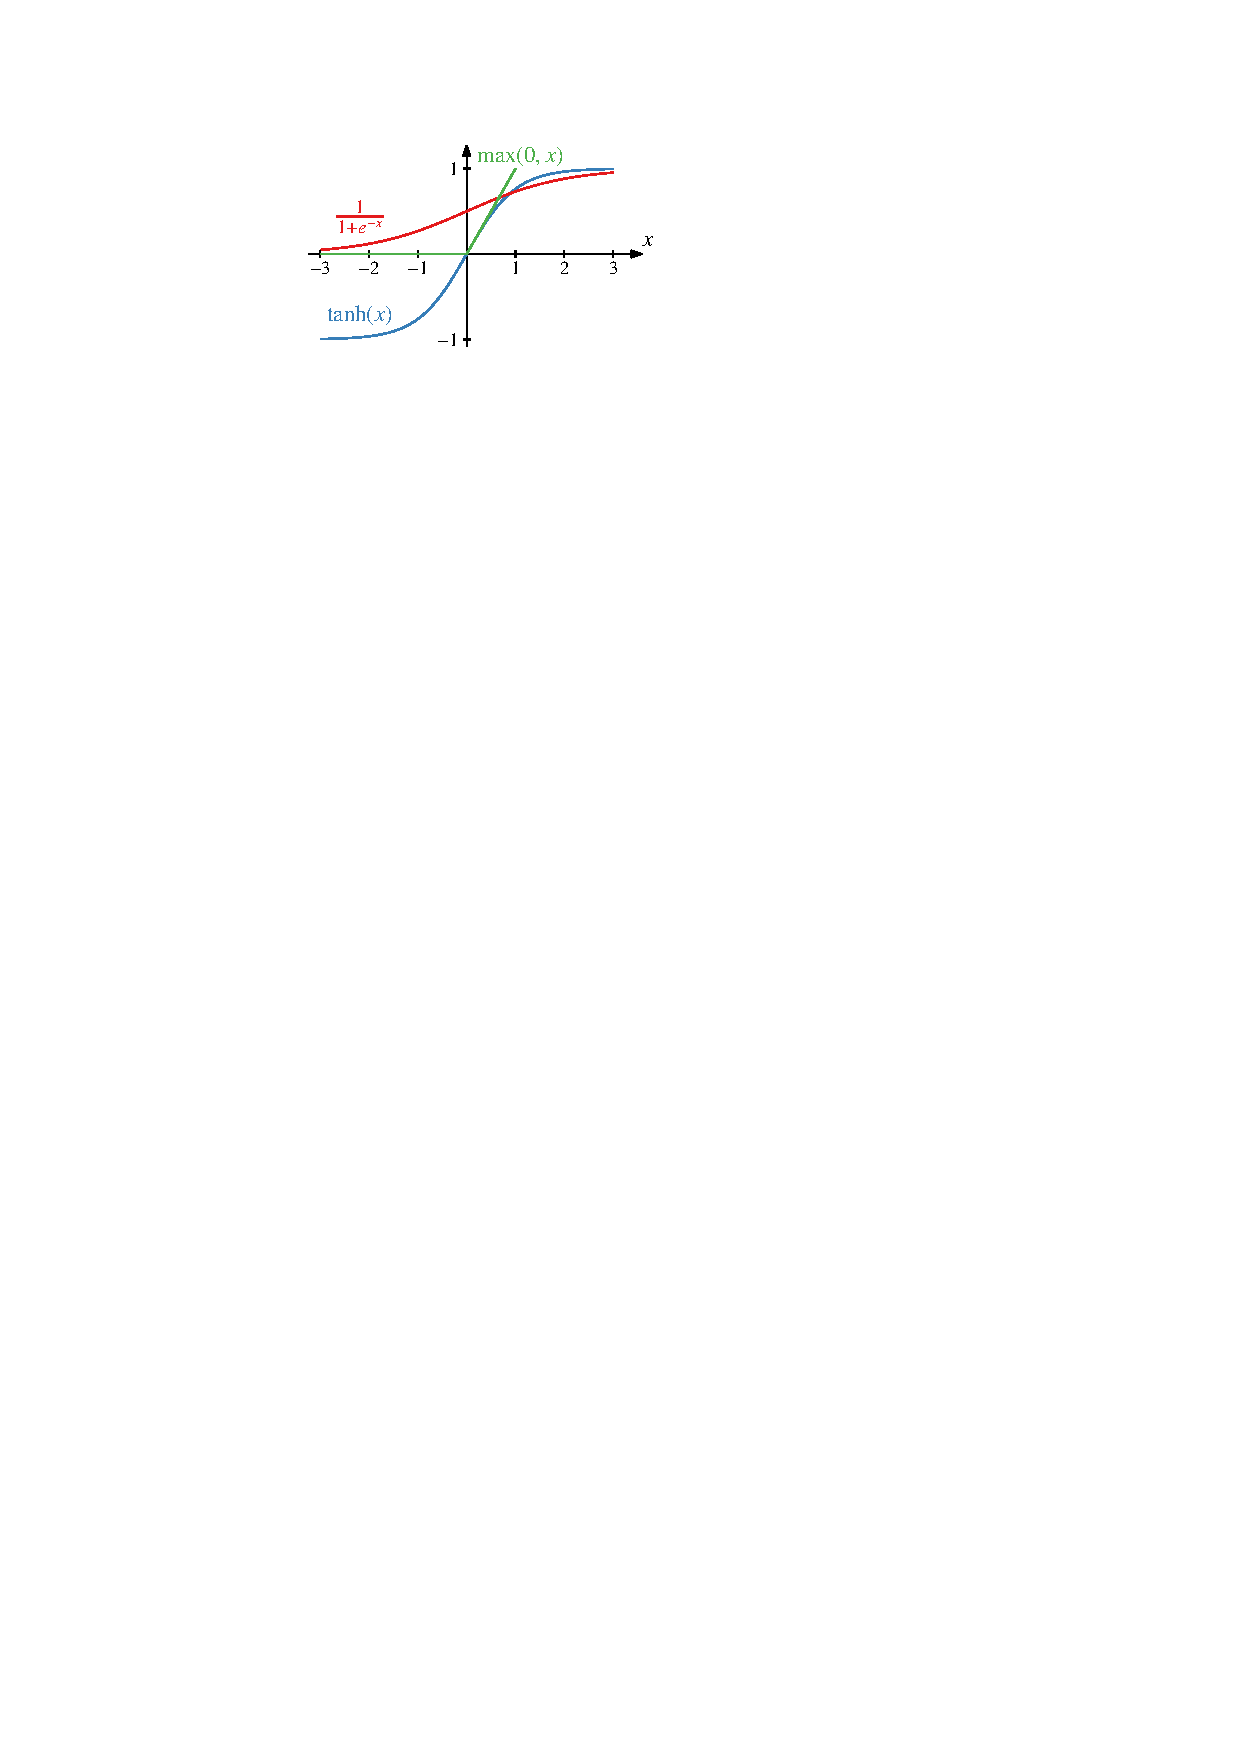
\includegraphics{./figures/theory/activation_functions.pdf}
    \subcaption{Commonly used activation functions for neural networks: logistic
      function (red), hyperbolic tangent (blue), and rectified linear unit --
      ReLU (green).}
    \label{fig:activation_functions}
  \end{subfigure}
  \caption{Feedforward neural network}
\end{figure}

\todo{$\varphi$ should be bold!}
Feedforward -> information flow from front to back.

An example of a simple feedforward neural networks is the multi-layer perceptron
consisting of a number of input neurons $\mathbf{x}$ that are used to feed the
discriminants to the network, a output layer with activation $\mathbf{y}$ and
several intermediate (hidden) layers connecting input and output layer. In
figure \ref{fig:multi_layer_perceptron} a multi-layer perceptron with a single
hidden layer is shown. Two layers of the network are connected by an affine
transformation $\mathbf{W}\mathbf{x} + \mathbf{b}$ and subsequent application of
an entry-wise \todo{non-linear and differentiable} activation function
$\bm{\varphi}$ (commonly called dense or densely-connected layers). The
activations of the neurons in the hidden layer $\mathbf{h}$ and the output layer
$\mathbf{y}$ for the case depicted in figure \ref{fig:multi_layer_perceptron}
are given by:
\begin{align*}
  &\mathbf{h} = \bm{\varphi}_{\text{h}}(\mathbf{W}_{\text{hx}} \mathbf{x} + \mathbf{b}_{\text{h}})
  &\mathbf{y} = \bm{\varphi}_{\text{y}}(\mathbf{W}_{\text{yh}} \mathbf{h} + \mathbf{b}_{\text{y}}) \eqdot
\end{align*}
Generally the sizes of the hidden layers as well as the choice of the activation
functions are hyperparameters of the model. The exception is the size of the
input and output layer which is given by the number of discriminants and the
number of outputs respectively. Moreover the activation function of the final
layer is determined by the underlying task. For binary classification the
logistic function $\sigma(x) = (1 + \exp(-x))^{-1}$ is applied to a single
output neuron giving the probability of an observation being of the positive
class. For multi-class classification the number of output neurons is equal to
the number of classes and \emph{softmax}
\begin{align*}
  \varphi_i(\mathbf{x}) = \frac{e^{x_i}}{\sum_j e^{x_j}}
\end{align*}
is commonly chosen as the activation function, where $\varphi_i(\mathbf{x})$ is
the activation of the $i$-th neuron and $x_i$ the value of the neuron before
activation. The \emph{softmax} function ensures that the sum of activations in a
layer equals one, such that the activations can be interpreted as class
probabilities. Further activation functions that are commonly used for the
intermediate layers are depicted in figure \ref{fig:activation_functions}.

There are numerous different layers and ways to interconnect them, which allows
for high flexibility when building networks.

Training:
\begin{itemize}
\item Weight initialisation
\item Loss functions
\item Backpropagation \cite{lecun-backprop}
\item Mini-batch Gradient Descent
\item Cross-Validation
\end{itemize}

For the training of neural networks a loss function that penalises errors in the
model's predictions is needed. In $K$-class classification tasks a commonly used
loss function is the categorical cross-entropy. For an observation of true class
$k \in \{ 1, \dots, K \}$ with discriminants $\mathbf{x}$ and a model
$\mathbf{p}(\mathbf{x})$ with per-class probabilities $p_k$ it is defined as
\begin{align*}
  L\left(k, \mathbf{p}(\mathbf{x}) \right) = - \log\left( p_k(\mathbf{x}) \right) \eqdot
\end{align*}
For binary classification it is sufficient to give the predicted probability $p$
for the positive class (e.g.\ an observation being signal) such that the binary
cross-entropy can be written as
\begin{align*}
  L(p(\mathbf{x})) = -t \, \log(p(\mathbf{x})) - (1 - t) \, \log(1 - p(\mathbf{x})) \eqcomma
\end{align*}
where $t$ is the binary indicator of the true class (0 for the negative and 1
for the positive class). When looking at a subset of observations with event
weights $w_i$ the loss $\mathcal{L}$ is defined as
\begin{align*}
  \mathcal{L} = \frac{\sum_i w_i L_i}{\sum_j w_j} \eqcomma
\end{align*}
which in case of the cross-entropy can be interpreted as the negative
log-likelihood of the model parameters given the observed subset of data. These
losses expect networks to predict probabilities which can be met if the
activation function of the final layer is the logistic function or softmax (eq.
\ref{eq:softmax}). The training process minimises the loss $\mathcal{L}$
(maximises the likelihood) with respect to the model parameters, i.e.\ the
weights and biases of the network, given the observed training data.

\todo{Find proper references} \cite{esl}

Large penalties to predictions
that are far off. Its better to be sort of off instead of completely off.
Motivate where in this thesis these loss functions are used. Both losses are
also called 'Log Loss'. $p$ should be a class probability. Perfect classifiers
have loss of zero. Last layer in neural network effectively does logistic
regression on the intermediate representation created from the previous layers.

\section{Recurrent Neural Networks}
\label{sec:rnn}

Recurrent: If a network has one or more cycles, that is, if it is possible to
follow a path from a unit back to itself.

Physics motivation: Able to do regression and classification on sequences of
physics objects like tracks, clusters, particle flow objects etc..

\subsection{Fully-Connected RNN}
\label{sec:fully_connected_rnn}

\todo{RNNs shown as an unfolded graph}

\textsc{Elman} network [Check Citation]\cite{elman, graves}:
% \textsc{Jordan} network \todo{look for citation}:
\begin{align*}
  \mathbf{c}_t &= \bm{\varphi}_{\text{c}}\left( \mathbf{W}_{\text{c}} \mathbf{x}_{t} + \mathbf{U}_{\text{c}} \mathbf{h}_{t-1} + \mathbf{b}_{\text{c}} \right) \\
  \mathbf{h}_t &= \bm{\varphi}_{\text{h}}\left( \mathbf{W}_{\text{h}} \mathbf{c}_{t} + \mathbf{b}_{\text{h}} \right)
\end{align*}
\todo{Should rename output $\mathbf{h}$ to $\mathbf{y}$ to be consistent.} with
trainable weights $\mathbf{W}$, recurrent weights $\mathbf{U}$ and biases
$\mathbf{b}$.

Key concepts: Due to recurrent links network has a form of memory and thus can
be context-dependent (recurrent connections allow a memory of the previous
inputs to persist in the internal state of the network [Graves
2012]\cite{graves}); Compared to MLP time affects processing instead of time
being parallelised into the spacial dimension;

Sequence of hidden activations and outputs can be calculated by recursively
applying the formulas while incrementing the timestep $t$.

At time $t=0$ the cell state is often set to zero (Graves 2012).

Vanishing gradient problem: Applying the sigmoid function multiple times leads
to vanishing gradients (plot?).

To be able to generalise to arbitrary length sequences the weights have to be
shared across all timesteps.

Trained using 'Backpropagation Through Time' i.e.\ repeated application of the
chain rule but now also considering that the weights are shared between
timesteps.

\subsection{Long Short-Term Memory}
\label{sec:lstm}

\begin{figure}[t]
  \centering
  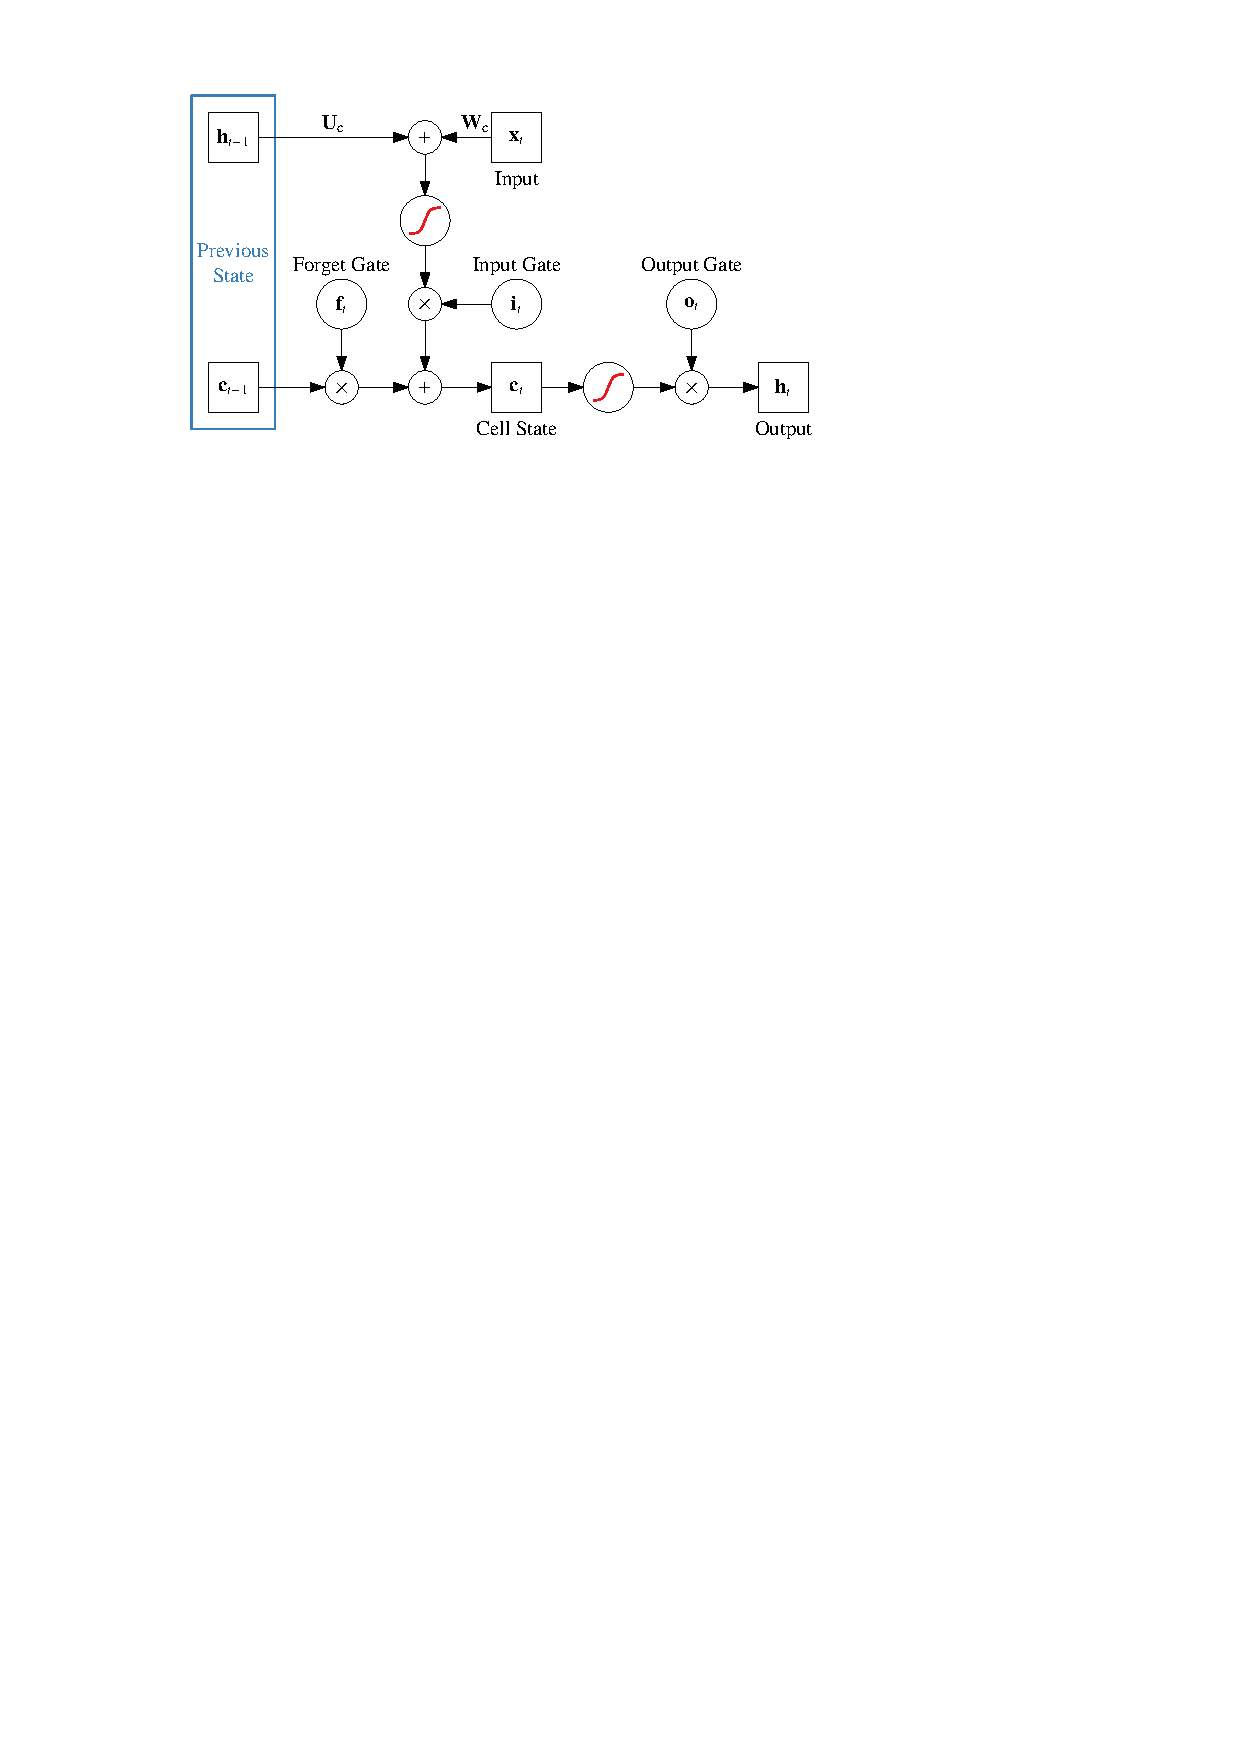
\includegraphics{./figures/theory/LSTM.pdf}
  \caption{Schematic description of a LSTM-cell.}
  \label{fig:schematic_lstm}
\end{figure}

[Check Citation]\cite{lstm}

\todo{Omit biases for brevity? Omit 'peephole' cite \cite{graves}}

Gate activations:
\begin{align*}
  \mathbf{f}_{t} &= \bm{\varphi}_{\text{g}}\left( \mathbf{W}_{\text{f}} \mathbf{x}_{t} + \mathbf{U}_{\text{f}} \mathbf{h}_{t-1} + \mathbf{b}_{\text{f}} \right) &
  \mathbf{i}_{t} &= \bm{\varphi}_{\text{g}}\left( \mathbf{W}_{\text{i}} \mathbf{x}_{t} + \mathbf{U}_{\text{i}} \mathbf{h}_{t-1} + \mathbf{b}_{\text{i}} \right) &
  \mathbf{o}_{t} &= \bm{\varphi}_{\text{g}}\left( \mathbf{W}_{\text{o}} \mathbf{x}_{t} + \mathbf{U}_{\text{o}} \mathbf{h}_{t-1} + \mathbf{b}_{\text{o}} \right)
\end{align*}
Cell state update:
\begin{align*}
  \mathbf{c}_{t} &= \mathbf{f}_{t} \circ \mathbf{c}_{t-1}
                   + \mathbf{i}_{t} \circ \bm{\varphi}_{\text{c}}(
                   \mathbf{W}_{\text{c}} \mathbf{x}_{t}+ \mathbf{U}_{\text{c}}
                   \mathbf{h}_{t-1} + \mathbf{b}_{\text{c}})
\end{align*}
Output:
\begin{align*}
  \mathbf{h}_{t} &= \mathbf{o}_{t} \circ \varphi_{\text{h}}(\mathbf{c}_{t})
\end{align*}

Stress that the gates depend on $x_t$ and $h_{t-1}$ via learn-able weights.
Therefore the inputting, outputting and forgetting is a learned process.

$\circ$: entry-wise product


Variables:
\begin{itemize}
\item $x_t$: input vector
\item $h_t$: output vector
\item $c_t$: cell state vector
\item $W$, $U$ and $b$: (recurrent -- $U$) weight matrices and bias vector
\item $f_t$, $i_t$ and $o_t$: gate vectors
  \begin{itemize}
  \item $f_t$: forget gate vector
  \item $i_t$: input gate vector
  \item $o_t$: output gate vector
  \end{itemize}
\end{itemize}

Activation functions:
\begin{itemize}
\item $\sigma_g$: element-wise sigmoid function (Gate activation -- recurrent
  activation)
\item $\sigma_c$: element-wise hyperbolic tangent (Cell activation -- recurrent
  activation)
\item $\sigma_h$: element-wise hyperbolic tangent (Output activation)
\end{itemize}

Gated Recurrent Unit (GRU) as an alternative.

Bidirectional Recurrent Neural Networks: consider past and future context when
classifying. Present the training sequence forwards and backwards to two
separate recurrent neural networks connected to the same output layer.

\section{Technical Setup}
\label{sec:tech_setup}

TMVA

Frameworks used for this thesis (theano \cite{theano}, keras \cite{keras})

Optimiser: Adam

Masking layer


%%% Local Variables:
%%% mode: latex
%%% TeX-master: "mythesis"
%%% End:
